\problemname{Bergsvandring}

\begin{figure}[ht!]
\centering
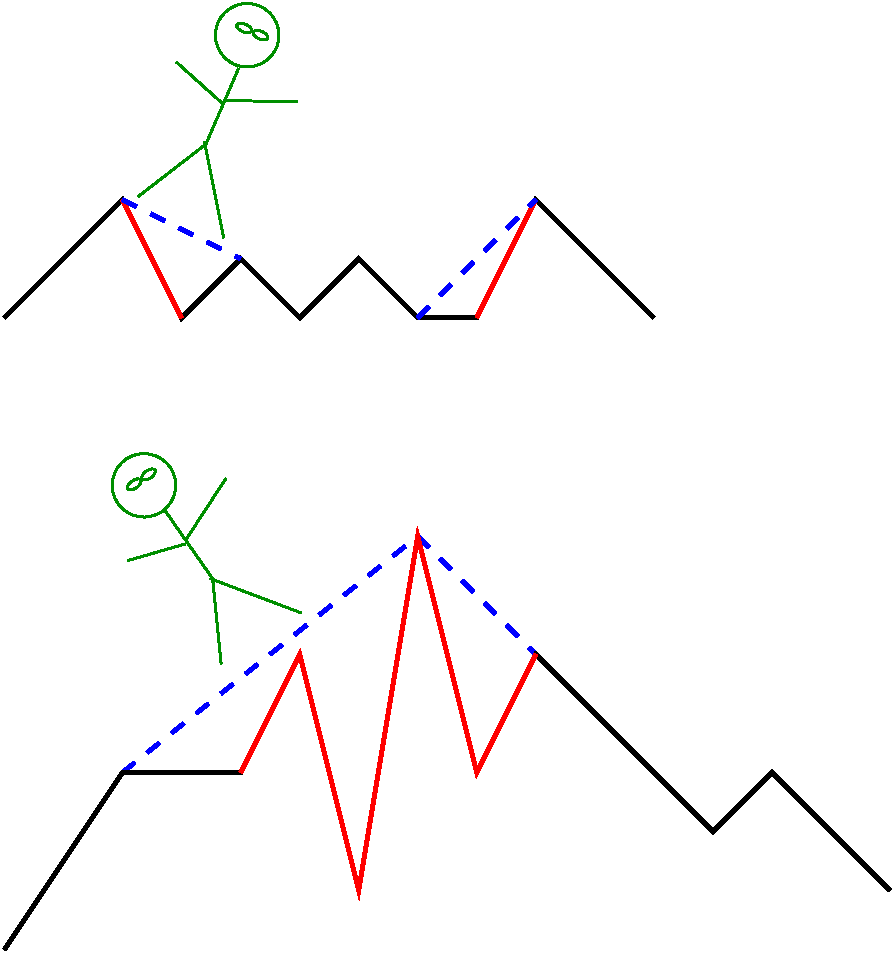
\includegraphics[width=0.4\textwidth]{berg.pdf}
\caption{Bergets utseende i exemplen. De röda segmenten har för hög lutning för att gå på. De streckade blå linjerna är broar som vandrarna bygger.}
\label{overflow}
\end{figure}

En bergskedja består av $n$ punkter, ($x_1$, $y_1$) till ($x_n$, $y_n$), där $x_1 < x_2 < ... < x_n$. Mellan punkt $i$ och punkt $i+1$ görs ett linjesegment.

Några vandrare vill ta sig över hela bergskedjan, dvs gå från punkt $1$ till punkt $n$. De kan dock inte gå på linjesegment om dess lutning är strikt större än $d$. Här definierar vi lutningen av linjen genom ($x_i$, $y_i$) och ($x_j$, $y_j$) som

$$
\frac{|y_i - y_j|}{|x_i - x_j|}
$$
där $|x|$ betecknar absolutvärdet av $x$.

För att göra vandringen möjlig kan de bygga broar i bergskedjan. En bro representeras också som ett linjesegment och byggs alltid mellan två punkter $i$ och $j$. En bro får självklart inte ha större lutning än $d$, och dessutom går det inte att bygga en bro som går igenom berget på något ställe.

Bestäm den minsta totala längden av de broar som behöver byggas för att vandringen ska vara möjlig.

\section*{Indata}
På först raden står heltalet $n$ och flyttalet $0 < d \le 10^5$, separerade av mellanslag.
De $n$ följande raderna innehåller två heltal $0 < x_i, y_i \le 10^5$, koordinaterna för punkt $i$, också separerade av mellanslag. Det är garanterat att $x_i < x_{i+1}$.

\section*{Utdata}
Skriv ut ett flyttal - minsta totala längden av broar som behövs för att göra vandringen möjlig.
Om det är omöjligt att utföra vandringen oavsett hur man bygger broarna, skriv istället ut $-1$.

\section*{Precision}
Ett svar på det här problemet kommer att räknas som korrekt om det absoluta felet är mindre än $10^{-3}$. Det är garanterat att resultatet för ett testfall inte påverkas av en \emph{liten} ändring av talet $d$ (detta för att undvika precisionsfel vid jämförelser av flyttal).

\section*{Poängsättning}

Din lösning kommer att testas på en mängd testfallsgrupper. För att få poäng för en grupp
så måste du klara alla testfall i gruppen.

\begin{tabular}{| l | l | l | l |}
\hline
Grupp & Poängvärde & Gränser \\ \hline
1     & 40         & $ 2 \le n \le 100$ \\ \hline
2     & 60         & $ 2 \le n \le 1\,000$ \\ \hline
\end{tabular}
